% -----------------------------------------  
% Autogenerated LaTeX file from XML DocBook  
% -----------------------------------------  
%%<params>
%%</params>
\documentclass[letterpaper,10pt,twoside,openright]{book}
\IfFileExists{ifxetex.sty}{%
    \usepackage{ifxetex}%
  }{%
    \newif\ifxetex
    \xetexfalse
  }
  \ifxetex
\usepackage{fontspec}
\usepackage{xltxtra}
\setmainfont{DejaVu Serif}
\setsansfont{DejaVu Sans}
\setmonofont{DejaVu Sans Mono}
\else
\usepackage[T1]{fontenc}
\usepackage[latin1]{inputenc}
\fi
\usepackage{fancybox}
\usepackage{makeidx}
\usepackage[hyperlink]{cll}
\renewcommand{\DBKreleaseinfo}{}
\renewcommand{\DBKrevhistory}{}
\setcounter{tocdepth}{5}
\setcounter{secnumdepth}{5}
\def\DBKcopyright{\noindent Copyright \textnormal{\copyright} Test Copyright Year 2014 Test Copyright Holder}


\def\DBKsubtitle{Test Subtitle}



\title{The Complete Lojban Language}
\author{AuthorFirstName AuthorSurName}
\hypersetup{%
pdfcreator={DBLaTeX-0.3.4},%
pdftitle={The Complete Lojban Language},%
pdfauthor={AuthorFirstName AuthorSurName}%
}
\renewcommand{\DBKindexation}{}
\makeindex
\makeglossary
\begin{document}
\lstsetup
\frontmatter
\maketitle
\tableofcontents
\mainmatter

% ------- 
% Chapter 
% ------- 

\chapter{COVERAGE: FULL}
\label{chapter-tour}\hyperlabel{chapter-tour}%
    
\noindent\begin{minipage}[c]{\linewidth}
\begin{center}
\imgexists{media/chapter-tour.gif}{{\imgevalsize{media/chapter-tour.gif}{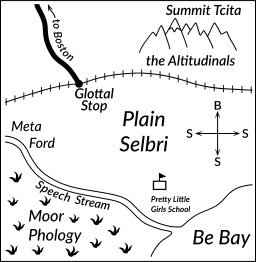
\includegraphics[width=\imgwidth,height=\imgheight,keepaspectratio=true]{media/chapter-tour.gif}}}}{}\end{center}
\end{minipage}

  
\section{The concept of the bridi}
\label{section-bridi}\hyperlabel{section-bridi}%
    
 \index{bridi!concept of} This chapter gives diagrammed examples of basic Lojban sentence structures. The most general pattern is covered first, followed by successive variations on the basic components of the Lojban sentence. There are many more capabilities not covered in this chapter, but covered in detail in later chapters, so this chapter is a 
 “quick tour” of the material later covered more slowly throughout the book. It also introduces most of the Lojban words used to discuss Lojban grammar.
  
    Let us consider John and Sam and three statements about them:
   
\begin{longfloat}{example}{\caption[{    }]{  \index{father!example}  \index{John and Sam!example}   \label{c2e1d1}\hyperlabel{c2e1d1}  }
\label{example-random-id-qIuj}\hyperlabel{example-random-id-qIuj}%
}

John is the father of Sam.

\end{longfloat}
  
\begin{longfloat}{example}{\caption[{    }]{  \index{hits!example}  \index{John and Sam!example}   \label{c2e1d2}\hyperlabel{c2e1d2}  }
\label{example-random-id-qiuQ}\hyperlabel{example-random-id-qiuQ}%
}

John hits Sam.

\end{longfloat}
  
\begin{longfloat}{example}{\caption[{    }]{  \index{taller!example}  \index{John and Sam!example}   \label{c2e1d3}\hyperlabel{c2e1d3}  }
\label{example-random-id-qIuS}\hyperlabel{example-random-id-qIuS}%
}

John is taller than Sam.

\end{longfloat}
  
 \index{sumti!relation with bridi} \index{brivla!relation to bridi} \index{predication!compared with bridi} \index{bridi!compared with predication} \index{predication!as a relationship} \index{relationship!active/static/attributive compared} These examples all describe relationships between John and Sam. However, in English, we use the noun 
  “father” to describe a static relationship in 
 Example \ref{example-random-id-qIuj}, the verb 
 “hits” to describe an active relationship in 
  Example \ref{example-random-id-qiuQ}, and the adjective 
 “taller” to describe an attributive relationship in 
  Example \ref{example-random-id-qIuS}. In Lojban we make no such grammatical distinctions; these three sentences, when expressed in Lojban, are structurally identical. The same part of speech is used to represent the relationship. In formal logic this whole structure is called a 
 “predication”; in Lojban it is called a 
 \hyperlink{valsi-bridi}{\emph{\emph{\index{bridi}bridi}}}, and the central part of speech is the 
 \hyperlink{valsi-selbri}{\emph{\emph{\index{selbri}selbri}}}. Logicians refer to the things thus related as 
 “arguments”, while Lojbanists call them 
 \hyperlink{valsi-sumti}{\emph{\emph{\index{sumti}sumti}}}. These Lojban terms will be used for the rest of the book.
  
\noindent\begin{minipage}[c]{\linewidth}
\begin{center}
\imgexists{media/chapter-2-diagram.png}{{\imgevalsize{media/chapter-2-diagram.png}{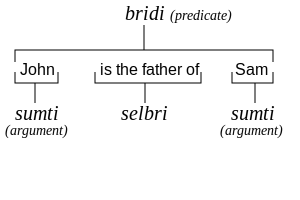
\includegraphics[width=\imgwidth,height=\imgheight,keepaspectratio=true]{media/chapter-2-diagram.png}}}}{}\end{center}
\end{minipage}

    
\section{Pronunciation}
\label{section-pronunciation}\hyperlabel{section-pronunciation}%
    
 \index{pronunciation!quick-{}tour version} Detailed pronunciation and spelling rules are given in 
 Chapter \ref{chapter-tour}, but what follows will keep the reader from going too far astray while digesting this chapter.
  
 \index{vowels!pronunciation of!quick-{}tour version} Lojban has six recognized vowels: 
 \emph{a}, 
 \emph{e}, 
 \emph{i}, 
 \emph{o}, 
 \emph{u} and 
 \emph{y}. The first five are roughly pronounced as 
 “a” as in 
 “father”, 
 \emph{e} as in 
 “let”, 
 \emph{i} as in 
 “machine”, 
 \emph{o} as in 
 “dome” and 
 \emph{u} as in 
 “flute”. 
 \emph{y} is pronounced as the sound called 
 “schwa”, that is, as the unstressed 
 “a” as in 
 “about” or 
 “around”.
  
 \index{diphthongs!pronunciation of!quick-{}tour version} The Lojban diphthongs 
 \emph{ai}, 
 \emph{ei}, 
 \emph{oi}, and 
 \emph{au} are pronounced much as in the English words 
 “sigh”, 
 “say”, 
 “boy”, and 
 “how”. Other Lojban diphthongs begin with an 
 \emph{i} pronounced like English 
 “y” (for example, 
 \emph{io} is pronounced 
 “yo”) or else with a 
 \emph{u} pronounced like English 
 “w” (for example, 
 \emph{ua} is pronounced 
 “wa”).
    
\section{Words that can act as sumti}
\label{section-sumti-cmavo}\hyperlabel{section-sumti-cmavo}%
    
 \index{pro-{}sumti!quick-{}tour version} Here is a short table of single words used as sumti. This table provides examples only, not the entire set of such words, which may be found in 
 Section \ref{section-bridi}.
  
\begin{tabulary}{\linewidth}{LL}
{}\emph{mi}&
{}
I/me, we/us
\tabularnewline
{}\emph{do}&
{}
you
\tabularnewline
{}\emph{ti}&
{}
this, these
\tabularnewline
{}\emph{ta}&
{}
that, those
\tabularnewline
{}\emph{tu}&
{}
that far away, those far away
\tabularnewline
{}\emph{zo'e}&
{}
unspecified value (used when a sumti is unimportant or obvious)
\tabularnewline
\end{tabulary}
    
\section{Some Selbri}
\label{section-some-selbri}\hyperlabel{section-some-selbri}%
    
\begin{tabulary}{\linewidth}{LL}
{}\hyperlink{valsi-vecnu}{\emph{\emph{\index{vecnu}vecnu}}}&
x1 (seller) sells x2 (goods) to x3 (buyer) for x4 (price)\tabularnewline
{}\hyperlink{valsi-tavla}{\emph{\emph{\index{tavla}tavla}}}&
x1 (talker) talks to x2 (audience) about x3 (topic) in language x4\tabularnewline
\end{tabulary}
  
\begin{longfloat}{example}{\caption[{  }]{  \label{c2e5d4}\hyperlabel{c2e5d4}  }
\label{example-random-id-k01t}\hyperlabel{example-random-id-k01t}%
}

\begin{tabulary}{\linewidth}{LLLLLL}
{}\ul{x1}&
{}
cu
&
{}\bf{tavla}&
{}\ul{x2}&
{}\ul{x3}&
{}\ul{x4}\tabularnewline
\end{tabulary}

\end{longfloat}
   
% ------- 
% Chapter 
% ------- 

\chapter{As Easy As A-{}B-{}C? The Lojban Letteral System And Its Uses}
\label{chapter-letterals}\hyperlabel{chapter-letterals}%
    
\noindent\begin{minipage}[c]{\linewidth}
\begin{center}
\imgexists{media/chapter-letterals.gif}{{\imgevalsize{media/chapter-letterals.gif}{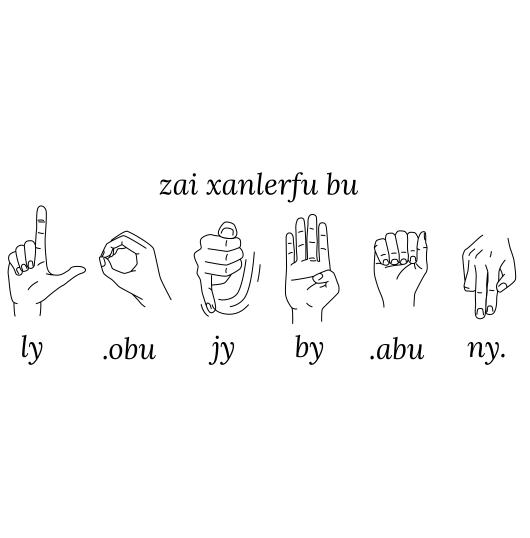
\includegraphics[width=\imgwidth,height=\imgheight,keepaspectratio=true]{media/chapter-letterals.gif}}}}{}\end{center}
\end{minipage}

  
\section{A to Z in Lojban, plus one}
\label{section-lerfu-liste}\hyperlabel{section-lerfu-liste}%
    
 \index{lerfu words!Lojban coverage requirement} The first requirement of a system of lerfu words for any language is that they must represent the lerfu used to write the language. The lerfu words for English are a motley crew: the relationship between 
 “doubleyou” and 
 “w” is strictly historical in nature; 
 “aitch” represents 
 “h” but has no clear relationship to it at all; and 
 “z” has two distinct lerfu words, 
 “zee” and 
 “zed”, depending on the dialect of English in question.
  
 \index{lerfu word!for "'"} \index{lerfu words!for consonants} \index{lerfu words!for vowels} \index{lerfu words!formation rules} All of Lojban's basic lerfu words are made by one of three rules:
  
\begin{tabulary}{\linewidth}{LLL}
{}\emph{.ua}&
{}
discovery
&
{}
confusion
\tabularnewline
\end{tabulary}
  \begin{itemize}

\item{}  to get a lerfu word for a vowel, add 
 \hyperlink{valsi-bu}{\emph{\emph{\index{bu}bu}}};
  

\item{}  to get a lerfu word for a consonant, add 
 \emph{y};
  

\item{}  the lerfu word for 
 \emph{'} is 
 \hyperlink{valsi-yhy}{\emph{\emph{\index{.y'y}.y'y}}}.
  
\end{itemize}
  
Consider the sentence
  \begin{quote}

Living things are made from cells.

\end{quote}
  
This cannot be correctly expressed as:
  
 \index{Tolkien!and non-{}standard Lojban orthography} \index{non-{}standard orthographies!Tengwar} Finally, an orthography using the Tengwar of Féanor, a fictional orthography invented by J. R. R. Tolkien and described in the Appendixes to 
   \emph{The Lord Of The Rings}, has been devised for Lojban. The following mapping, which closely resembles that used for Westron, will be meaningful only to those who have read those appendixes. In brief, the tincotéma and parmatéma are used in the conventional ways; the calmatéma represents palatal consonants, and the quessetéma represents velar consonants.
   
\noindent
\begin{description}
\item[{tinco}] \emph{t}
\item[{calma}] -{}
\end{description}
  
\begin{longfloat}{example}{\caption[{    }]{  \index{syllabic pronunciations of consonants!in fu'ivla category attachment!example} \index{syllabic pronunciations of consonants!in fu'ivla!example}  \label{c4e7d8}\hyperlabel{c4e7d8}  }
\label{example-random-id-FTfQ}\hyperlabel{example-random-id-FTfQ}%
}

\begin{tabulary}{\linewidth}{L}
\multicolumn{1}{l}{
자모 \emph{from Korean}
}\tabularnewline
\multicolumn{1}{l}{
djamo \emph{Lojbanize}
}\tabularnewline
\multicolumn{1}{l}{
lerf,r,djamo \emph{prefix rafsi}
}\tabularnewline
\multicolumn{1}{l}{
ler,l,djamo \emph{prefix rafsi}
}\tabularnewline
\end{tabulary}

\end{longfloat}
  
\noindent
\begin{description}
\item[{\hyperlink{valsi-jungo}{\emph{\emph{\index{jungo}jungo}}}}] Chinese (from “Zhong $^{\text{1}}$ guo $^{\text{2}}$”)
\end{description}
  
\noindent
\begin{description}
\item[{\hyperlink{valsi-dotco}{\emph{\emph{\index{dotco}dotco}}}}] German (from „Deutsch“)
\item[{\hyperlink{valsi-fraso}{\emph{\emph{\index{fraso}fraso}}}}] French (from « Français »)
\item[{\hyperlink{valsi-xurdo}{\emph{\emph{\index{xurdo}xurdo}}}}] Urdu
\end{description}
  
\begin{tabulary}{\linewidth}{LL}
{}\emph{bai}&
{}
bapli
\tabularnewline
\end{tabulary}
  
\begin{tabulary}{\linewidth}{LLLLL}
construct&
afterthought logical&
forethought logical&
afterthought non-logical&
forethought non-logical\tabularnewline
\hline
bridi&
{}\hyperlink{section-pronunciation}{ijek*}&
{}\hyperlink{section-bridi}{gek}&
{}\hyperlink{section-mekso-numbers}{ijoik*}&
{}\hyperlink{section-mekso-numbers}{joigik}\tabularnewline
\end{tabulary}
  \begin{enumerate}

\item{}  Change double consonants other than 
 \emph{cc} to single consonants.
  

\item{}  Change 
 \emph{cc} before a front vowel to 
 \emph{kc}, but otherwise to 
 \emph{k}.
  
\end{enumerate}
  
\noindent
\begin{description}
\item[{ROI}]   objective quantified tense flag
  
\begin{tabulary}{\linewidth}{LL}
{}\emph{paroi}&
{}
once
\tabularnewline
{}
[N]roi
&
{}
[N] times
\tabularnewline
\end{tabulary}
  \end{description}
  
\begin{tabulary}{\linewidth}{LLLL}
{}\emph{ba'i}&
{}
basti
&
{}
replaced by
&
{}
instead of
\tabularnewline
{}\emph{bai}&
{}
bapli
&
{}
compelled by
&
{}
compelling
\tabularnewline
\end{tabulary}
  
\begin{tabulary}{\linewidth}{LLLL}
{}\emph{vo'a}&
{}
KOhA
&
{}
vo'a-{}series
&
{}
x1 of this bridi 
\tabularnewline
\end{tabulary}
  \begin{enumerate}

\item{}  Count the total number of letters, including hyphens and apostrophes; call it 
 \texttt{L}.
  

\item{}  Count the number of apostrophes; call it 
 \texttt{A}.
  
\end{enumerate}
  
\begin{tabulary}{\linewidth}{L}
\multicolumn{1}{l}{
soirsai
}\tabularnewline
\multicolumn{1}{l}{
sonci sanmi
}\tabularnewline
\multicolumn{1}{l}{
soldier meal
}\tabularnewline
\multicolumn{1}{l}{
field rations
}\tabularnewline
\end{tabulary}
  
\begin{longfloat}{example}{\caption[{  }]{  \label{c4e12d1}\hyperlabel{c4e12d1}  }
\label{example-random-id-qJKu}\hyperlabel{example-random-id-qJKu}%
}

\begin{tabulary}{\linewidth}{L}
\multicolumn{1}{l}{
zbasai
}\tabularnewline
\multicolumn{1}{l}{\emph{zba + sai}}\tabularnewline
\multicolumn{1}{l}{
(1000 * 6) -{} (500 * 0) + (100 * 0) -{} (10 * 15) -{} 3 = 5847
}\tabularnewline
\end{tabulary}

\end{longfloat}
  
\begin{tabular*}{\linewidth}{llll}
{\emph{-{}ger-{}}, } & {\emph{-{}ge'u-{}}, } & {\emph{-{}gerk-{}}, } & {\emph{-{}gerku}} \\

\end{tabular*}
  
\begin{longfloat}{example}{\caption[{  }]{  \label{c4e5d6}\hyperlabel{c4e5d6}  }
\label{example-random-id-aiAR}\hyperlabel{example-random-id-aiAR}%
}

\begin{tabulary}{\linewidth}{L}
\multicolumn{1}{l}{
bralo'i
}\tabularnewline
\multicolumn{1}{l}{
big-{}boat
}\tabularnewline
\multicolumn{1}{l}{
ship
}\tabularnewline
\end{tabulary}

\end{longfloat}
  
\begin{longfloat}{example}{\caption[{   }]{   \index{Old McDonald!example}    \label{c3e3d1}\hyperlabel{c3e3d1}  }
\label{example-random-id-k2B4}\hyperlabel{example-random-id-k2B4}%
}
\begin{itemize}

\item{}.i.ai.i.ai.o


\item{}[ʔi ʔaj ʔi ʔaj ʔo]


\item{}Ee! Eye! Ee! Eye! Oh!

\end{itemize}

\end{longfloat}
  \begin{quote}

  \begin{itemize}

\item{}               [se] JOI  [nai]
 
  

\item{}               [se] BIhI [nai]
 
  

\item{}               GAhO [se] BIhI [nai] GAhO
 
  
\end{itemize}
  

\end{quote}
  
\begin{longfloat}{example}{\caption[{  }]{  \label{c14e13d15}\hyperlabel{c14e13d15}  }
\label{example-random-id-HyVv}\hyperlabel{example-random-id-HyVv}%
}

  \emph{ni$^{\text{3}}$ zou$^{\text{3}}$ hai$^{\text{2}}$shi pao$^{\text{3}}$}  

\end{longfloat}
  
    must always be an insect with large brightly-{}colored wings, of the family 
 \emph{Lepidoptera}.
  \begin{quote}

  \hyperlink{valsi-dunda}{\emph{\emph{\index{dunda}dunda}}} x1 gives x2 to x3  

\end{quote}
  
\begin{tabulary}{\linewidth}{LL}
{}
nairu'e
&
{}

\tabularnewline
{}
naisai
&
{}

\tabularnewline
{}
naicai
&
{}

\tabularnewline
\end{tabulary}
  
\begin{longfloat}{example}{\caption[{  }]{  \label{c4e2d1}\hyperlabel{c4e2d1}  }
\label{example-random-id-qiXV}\hyperlabel{example-random-id-qiXV}%
}

\begin{tabular*}{\linewidth}{l}
{.iseci'i} \\
{.i se ci'i} \\

\end{tabular*}

\end{longfloat}
  
\begin{tabulary}{\linewidth}{LLL}
x1&
agent&
{}\hyperlink{valsi-mi}{\emph{\emph{\index{mi}mi}}}\tabularnewline
x2&
destination&
{}\emph{\index{la bastn.}la bastn.}\tabularnewline
x3&
origin&
{}\emph{\index{la .atlantas.}la .atlantas.}\tabularnewline
x4&
route&
{}\emph{\index{le dargu}le dargu}\tabularnewline
x5&
means&
{}\emph{\index{le karce}le karce}\tabularnewline
\end{tabulary}
  
 \index{stress!showing non-{}standard} \index{capital letters!use of} Capital letters are used only to represent non-{}standard stress, which can appear only in the representation of Lojbanized names. Thus the English name 
 “Josephine”, as normally pronounced, is Lojbanized as 
 \emph{DJOsefin.}, pronounced 
 ['dʒosɛfinʔ]. (See 
 Section \ref{section-some-selbri} for an explanation of the symbols within square brackets.) Technically, it is sufficient to capitalize the vowel letter, in this case 
  \emph{O}, but it is easier on the reader to capitalize the whole syllable.
  
 \index{lerfu words!table of Lojban} Therefore, the following table represents the basic Lojban alphabet:
    
\noindent
\begin{description}
\item[{\emph{'}}] \hyperlink{valsi-yhy}{\emph{\emph{\index{.y'y.}.y'y.}}}
\item[{\emph{a}}] \hyperlink{valsi-abu}{\emph{\emph{\index{.abu}.abu}}}
\item[{\emph{b}}] \hyperlink{valsi-by}{\emph{\emph{\index{by.}by.}}}
\end{description}
  
   \index{Spanish ch!example} \index{Spanish ll!example}  \index{compound letters!native language!representing as distinct letters} \index{accented letters!considered as distinct from unaccented} \index{diacritical marks!considered as forming distinct letters} Some languages, like Swedish and Finnish, consider certain accented lerfu to be completely distinct from their unaccented equivalents, but Lojban does not make a formal distinction, since the printed characters look the same whether they are reckoned as separate letters or not. In addition, some languages consider certain 2-{}letter combinations (like 
 “ll” and 
 “ch” in Spanish) to be letters; this may be represented by enclosing the combination in 
 \hyperlink{valsi-tei}{\emph{\emph{\index{tei}tei}}}…\hyperlink{valsi-foi}{\emph{\emph{\index{foi}foi}}}.
  
 \index{lerfu words!forming new for non-{}Lojban letters using bu} In addition, when discussing a specific language, it is permissible to make up new lerfu words, as long as they are either explained locally or well understood from context: thus Spanish 
 “ll” or Croatian 
 „lj“ could be called 
 \hyperlink{valsi-ibu}{\emph{\emph{\index{.ibu}.ibu}}}, but that usage would not necessarily be universally understood.
  
  Section \ref{section-lerfu-liste} contains a table of proposed lerfu words for some common accent marks.
   
\begin{longfloat}{example}{\caption[{   }]{  \label{c17e8d2}\hyperlabel{c17e8d2}  \index{Mitsubishi!example}  }
\label{example-random-id-pLUV}\hyperlabel{example-random-id-pLUV}%
}

\begin{tabulary}{\linewidth}{LLLLLLLLLL}
{}my.&
{}.ibu&
{}ty.&
{}sy.&
{}.ubu&
{}by.&
{}.ibu&
{}sy.&
{}.y'y.bu&
{}.ibu\tabularnewline
\multicolumn{10}{l}{
  “m”  “i”  “t”  “s”  “u”  “b”  “i”  “s”  “h”  “i”  
}\tabularnewline
\end{tabulary}

\end{longfloat}
  
\begin{longfloat}{example}{\caption[{  }]{  \label{c18e1d1}\hyperlabel{c18e1d1}  }
\label{example-random-id-dGcT}\hyperlabel{example-random-id-dGcT}%
}
3x + 2y
\end{longfloat}
  
 \index{mathematical notation!and omitted operators} contains omitted multiplication operators, but there are other possible interpretations for the strings 
  “3x” and 
 “2y” than as mathematical multiplication. Therefore, the Lojban verbal (spoken and written) form of 
  Example \ref{example-random-id-dGcT} must not omit the multiplication operators.
   
 \index{mekso chapter!completeness} \index{mekso chapter!table notation convention} The remainder of this chapter explains (in as much detail as is currently possible) the mekso system. This chapter is by intention complete as regards mekso components, but only suggestive about uses of those components – as of now, there has been no really comprehensive use made of mekso facilities, and many matters must await the test of usage to be fully clarified.
    
\section{Lojban numbers}
\label{section-mekso-numbers}\hyperlabel{section-mekso-numbers}%
    
The following cmavo are discussed in this section:
  
\begin{tabulary}{\linewidth}{LLL}
{}\emph{pa}&
{}
PA
&
{}
1
\tabularnewline
\end{tabulary}
  
 \index{hundred!expressing as number} \index{ten!expressing as number} \index{numbers!as compound cmavo} \index{digits!cmavo for} \index{numbers!expressing simple} The simplest kind of mekso are numbers, which are cmavo or compound cmavo. There are cmavo for each of the 10 decimal digits, and numbers greater than 9 are made by stringing together the cmavo. Some examples:
  
\begin{longfloat}{example}{\caption[{  }]{  \label{c18e2d3}\hyperlabel{c18e2d3}  }
\label{example-random-id-gjzw}\hyperlabel{example-random-id-gjzw}%
}

\begin{tabulary}{\linewidth}{LLLLLLLLLL}
{}pa&
{}re&
{}ci&
{}vo&
{}mu&
{}xa&
{}ze&
{}bi&
{}so&
{}no\tabularnewline
{}one&
{}two&
{}three&
{}four&
{}five&
{}six&
{}seven&
{}eight&
{}nine&
{}zero\tabularnewline
\multicolumn{10}{l}{1234567890}\tabularnewline
\multicolumn{10}{l}{
one billion, two hundred and thirty-{}four million, five hundred and sixty-{}seven thousand, eight hundred and ninety.
}\tabularnewline
\end{tabulary}

\end{longfloat}
      
\section{Test Selmaho}
\label{section-test-selmaho}\hyperlabel{section-test-selmaho}%
    
 \index{selma'o!cross-{}reference list of!selma'o catalog} The following paragraphs list all the selma'o of Lojban, with a brief explanation of what each one is about, and reference to the chapter number where each is explained more fully. As usual, all selma'o names are given in capital letters (with “h” serving as the capital of “'”) and are the names of a representative cmavo, often the most important or the first in alphabetical order. One example is given of each selma'o: for selma'o which have several uses, the most common use is shown.
  
\paragraph*{  \index{A!selma'o catalog} \index{connection!of sumti!selma'o catalog}  \label{A}\hyperlabel{A} selma'o A (Section \ref{section-mekso-numbers})
 }

\noindent
  
Specifies a logical connection (e.g. “and”, “or”, “if”), usually between sumti.
  
\begin{lstlisting}[firstnumber=1,]
      la djan. .a la djein. klama le zarci
      John and/or Jane goes to the store.
    \end{lstlisting}
   
Also used to create vowel lerfu words when followed with “bu”.
  
\paragraph*{  \index{BAI!selma'o catalog} \index{sumti place!additional!selma'o catalog}  \label{BAI}\hyperlabel{BAI} selma'o BAI (Section \ref{section-pronunciation})
 }

\noindent
   
May be prefixed to a sumti to specify an additional place, not otherwise present in the place structure of the selbri, and derived from a single place of some other selbri.
  
\begin{lstlisting}[firstnumber=1,]
      mi tavla bau la lojban.
      I speak in-language Lojban.
    \end{lstlisting}
   % --------	
% GLOSSARY	
% --------	

\chapter{Lojban Word Glossary}

All definitions in this glossary are brief and unofficial.
Only the published dictionary is a truly official reference for word
definitions.  These definitions are here simply as a quick reference.


\section*{A}

\noindent
\begin{description}
\item[\hypertarget{valsi-abu}{abu}]~ 

letteral for a.



\end{description}

\section*{B}

\noindent
\begin{description}
\item[\hypertarget{valsi-bridi}{bridi}]~ 

<{}inlinemath>{}x<{}subscript>{}1<{}/subscript>{}<{}/inlinemath>{} (text) is a predicate relationship with relation <{}inlinemath>{}x<{}subscript>{}2<{}/subscript>{}<{}/inlinemath>{} among arguments (sequence/set) <{}inlinemath>{}x<{}subscript>{}3<{}/subscript>{}<{}/inlinemath>{}.


\item[\hypertarget{valsi-bu}{bu}]~ 

convert any single word to BY.


\item[\hypertarget{valsi-by}{by}]~ 

letteral for b.



\end{description}

\section*{D}

\noindent
\begin{description}
\item[\hypertarget{valsi-dotco}{dotco}]~ 

<{}inlinemath>{}x<{}subscript>{}1<{}/subscript>{}<{}/inlinemath>{} reflects German/Germanic culture/nationality/language in aspect <{}inlinemath>{}x<{}subscript>{}2<{}/subscript>{}<{}/inlinemath>{}.


\item[\hypertarget{valsi-dunda}{dunda}]~ 

<{}inlinemath>{}x<{}subscript>{}1<{}/subscript>{}<{}/inlinemath>{} [donor] gives/donates gift/present <{}inlinemath>{}x<{}subscript>{}2<{}/subscript>{}<{}/inlinemath>{} to recipient/beneficiary <{}inlinemath>{}x<{}subscript>{}3<{}/subscript>{}<{}/inlinemath>{} [without payment/exchange].



\end{description}

\section*{F}

\noindent
\begin{description}
\item[\hypertarget{valsi-foi}{foi}]~ 

terminator: end composite lerfu; never elidable.


\item[\hypertarget{valsi-fraso}{fraso}]~ 

<{}inlinemath>{}x<{}subscript>{}1<{}/subscript>{}<{}/inlinemath>{} reflects French/Gallic culture/nationality/language in aspect <{}inlinemath>{}x<{}subscript>{}2<{}/subscript>{}<{}/inlinemath>{}.



\end{description}

\section*{I}

\noindent
\begin{description}
\item[\hypertarget{valsi-ibu}{ibu}]~ 

letteral for i.



\end{description}

\section*{J}

\noindent
\begin{description}
\item[\hypertarget{valsi-jungo}{jungo}]~ 

<{}inlinemath>{}x<{}subscript>{}1<{}/subscript>{}<{}/inlinemath>{} reflects Chinese [Mandarin, Cantonese, Wu, etc.] culture/nationality/language in aspect <{}inlinemath>{}x<{}subscript>{}2<{}/subscript>{}<{}/inlinemath>{}.



\end{description}

\section*{M}

\noindent
\begin{description}
\item[\hypertarget{valsi-mi}{mi}]~ 

pro-{}sumti: me/we the speaker(s)/author(s); identified by self-{}vocative.



\end{description}

\section*{S}

\noindent
\begin{description}
\item[\hypertarget{valsi-selbri}{selbri}]~ 

NO JBOVLASTE DEFINITION FOR "selbri" FOUND!


\item[\hypertarget{valsi-sumti}{sumti}]~ 

<{}inlinemath>{}x<{}subscript>{}1<{}/subscript>{}<{}/inlinemath>{} is a/the argument of predicate/function <{}inlinemath>{}x<{}subscript>{}2<{}/subscript>{}<{}/inlinemath>{} filling place <{}inlinemath>{}x<{}subscript>{}3<{}/subscript>{}<{}/inlinemath>{} (kind/number).



\end{description}

\section*{T}

\noindent
\begin{description}
\item[\hypertarget{valsi-tavla}{tavla}]~ 

<{}inlinemath>{}x<{}subscript>{}1<{}/subscript>{}<{}/inlinemath>{} talks/speaks to <{}inlinemath>{}x<{}subscript>{}2<{}/subscript>{}<{}/inlinemath>{} about subject <{}inlinemath>{}x<{}subscript>{}3<{}/subscript>{}<{}/inlinemath>{} in language <{}inlinemath>{}x<{}subscript>{}4<{}/subscript>{}<{}/inlinemath>{}.


\item[\hypertarget{valsi-tei}{tei}]~ 

composite letteral follows; used for multi-{}character letterals.



\end{description}

\section*{V}

\noindent
\begin{description}
\item[\hypertarget{valsi-vecnu}{vecnu}]~ 

<{}inlinemath>{}x<{}subscript>{}1<{}/subscript>{}<{}/inlinemath>{} [seller] sells/vends <{}inlinemath>{}x<{}subscript>{}2<{}/subscript>{}<{}/inlinemath>{} [goods/service/commodity] to buyer <{}inlinemath>{}x<{}subscript>{}3<{}/subscript>{}<{}/inlinemath>{} for amount/cost/expense <{}inlinemath>{}x<{}subscript>{}4<{}/subscript>{}<{}/inlinemath>{}.



\end{description}

\section*{X}

\noindent
\begin{description}
\item[\hypertarget{valsi-xurdo}{xurdo}]~ 

<{}inlinemath>{}x<{}subscript>{}1<{}/subscript>{}<{}/inlinemath>{} reflects Urdu language/culture/nationality in aspect <{}inlinemath>{}x<{}subscript>{}2<{}/subscript>{}<{}/inlinemath>{}.



\end{description}

\section*{Y}

\noindent
\begin{description}
\item[\hypertarget{valsi-yhy}{y'y}]~ 

letteral for '.



\end{description}
\printindex

\end{document}
